\section{Experimental validation}\label{sec:experiments}

So far, the functional basis of \method has been implemented in its web version.
The most relevant partial result is the consolidation of a complete flow, still under validation, that goes from the creation of a geographic project to the generation of a preliminary sewer network processed by graph algorithms.
The current version already allows users to create and list projects, open the editor, visualize streets and nodes, edit the graph, run the pipeline, save the processed network, and reload the persisted state.
Figure~\ref{fig:before-after-processing} shows a local example of this transformation, comparing the enriched editable graph before processing with the directed network produced after the pipeline.

\begin{figure}[ht]
\centering
    \begin{minipage}{.49\linewidth}
    \centering
    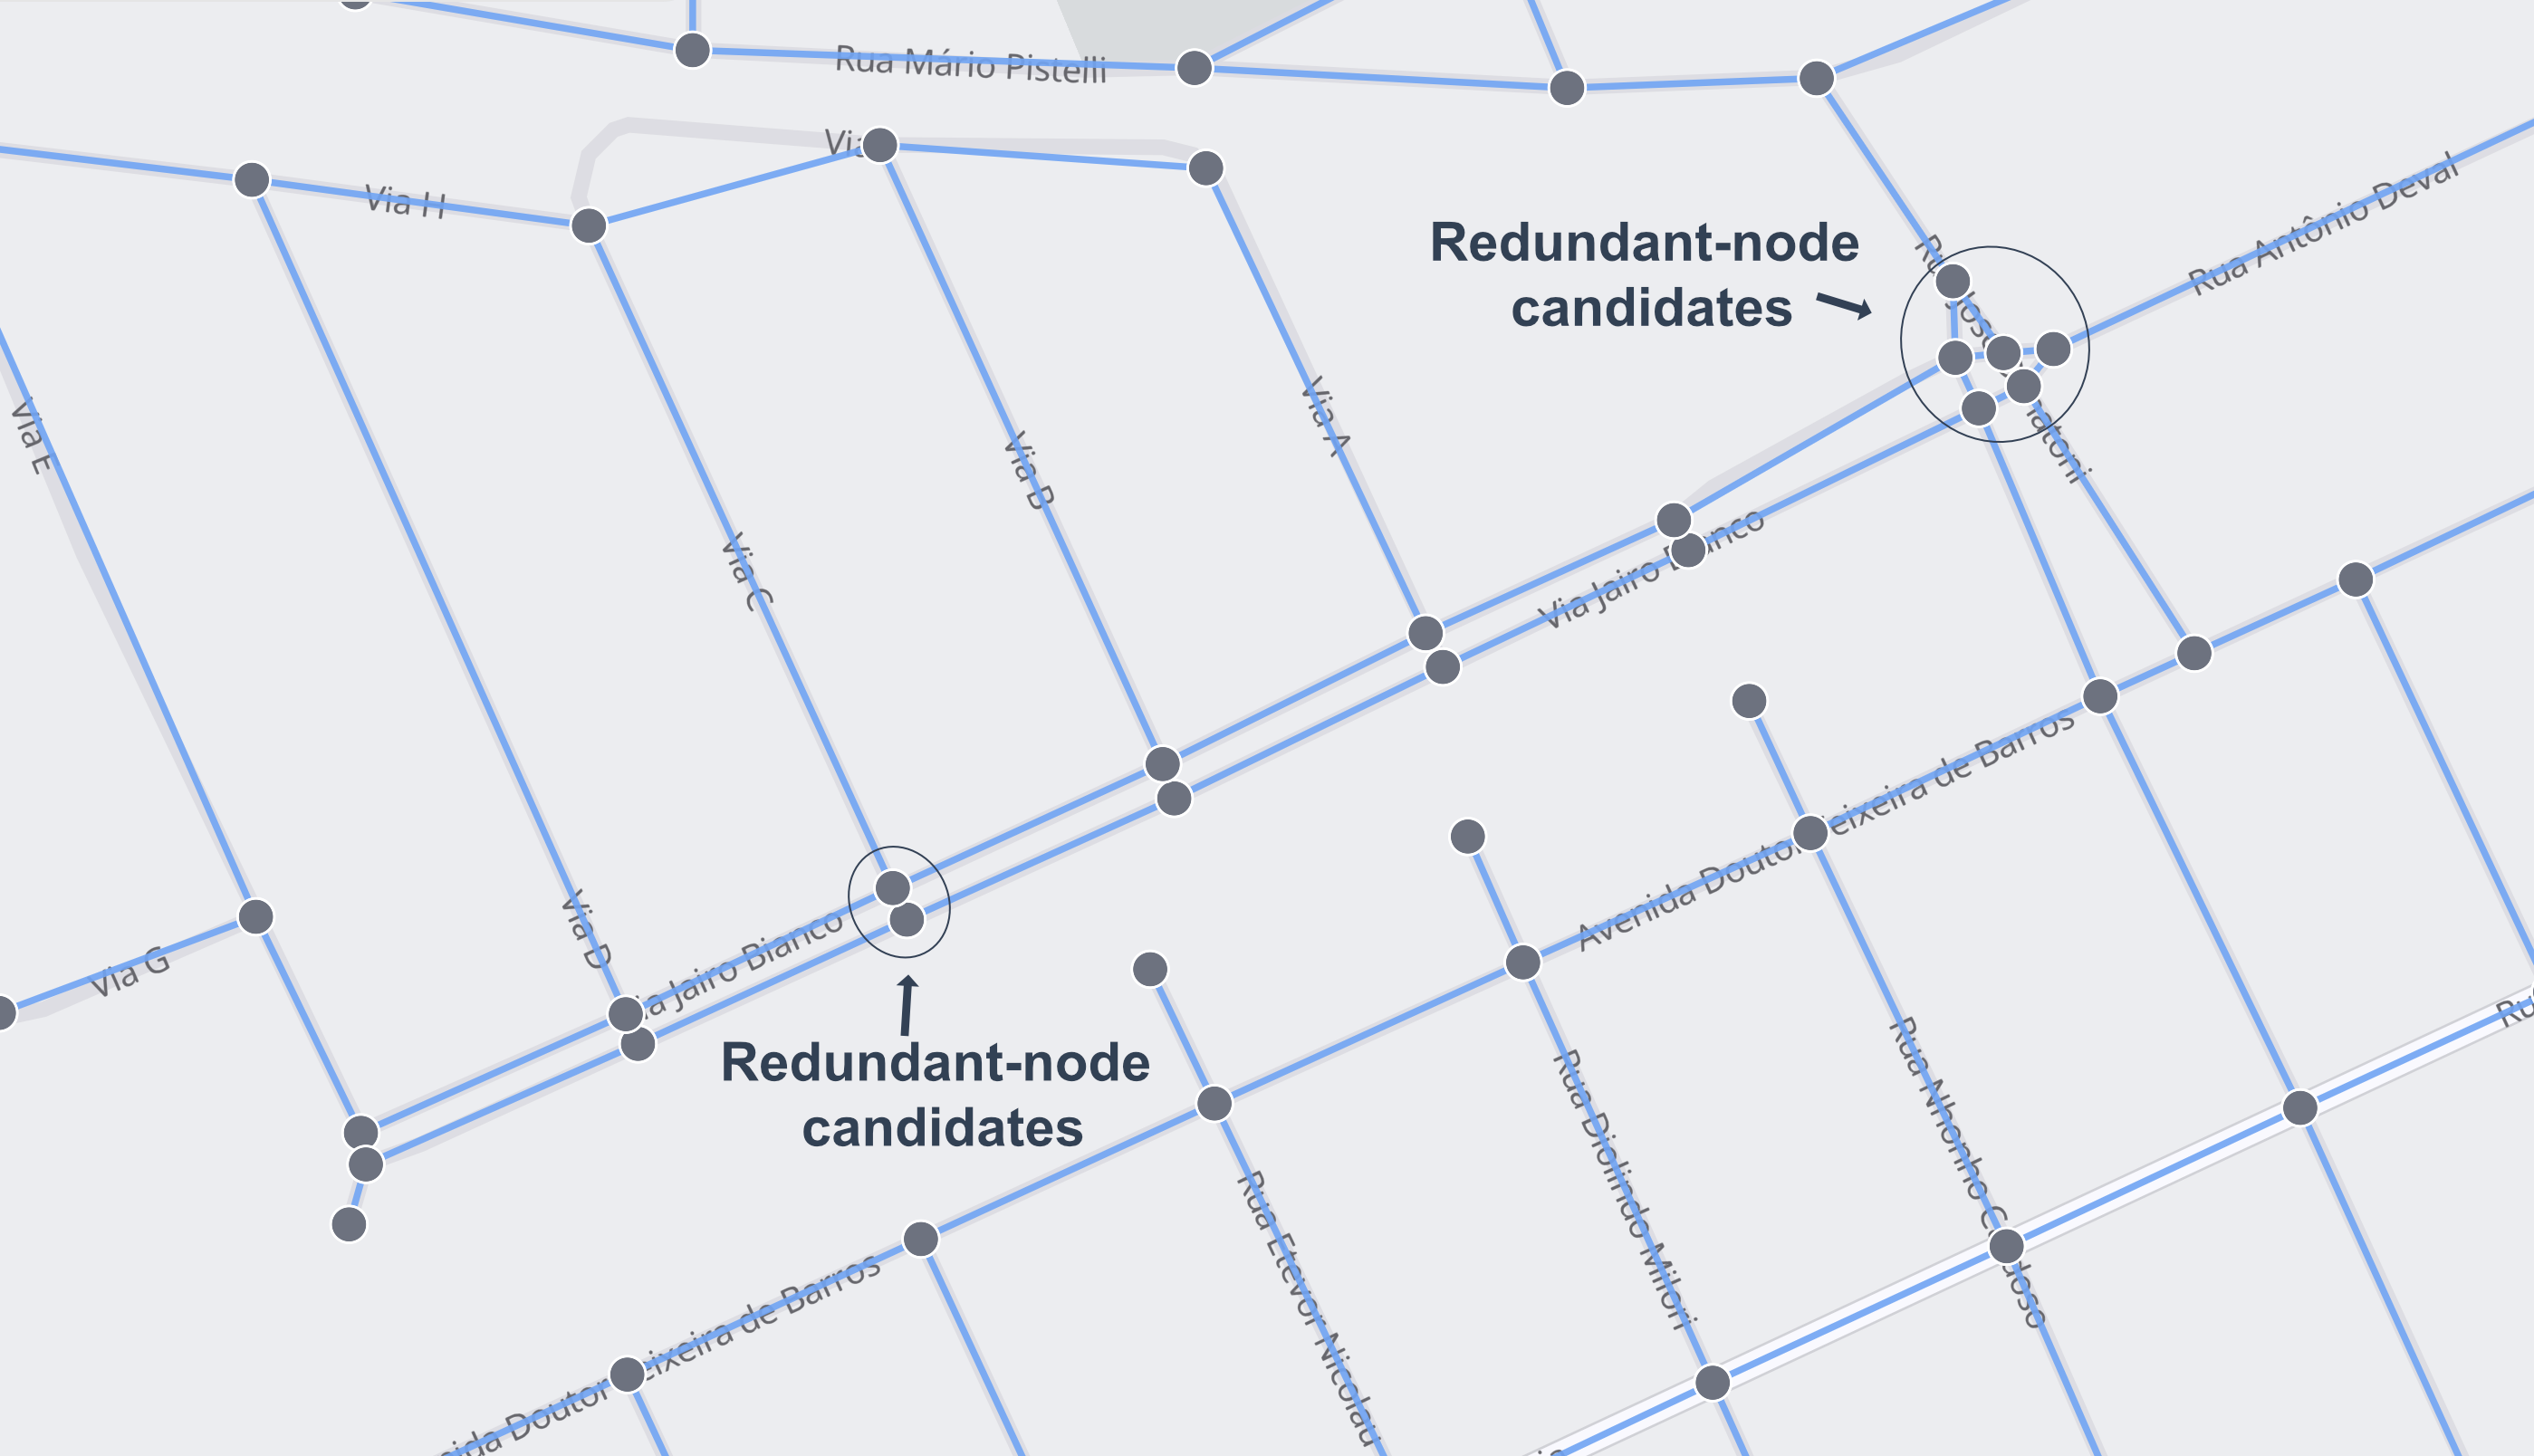
\includegraphics[width=\linewidth]{images/pre-processed.png}
    \end{minipage}
\hfill
    \begin{minipage}{.49\linewidth}
    \centering
    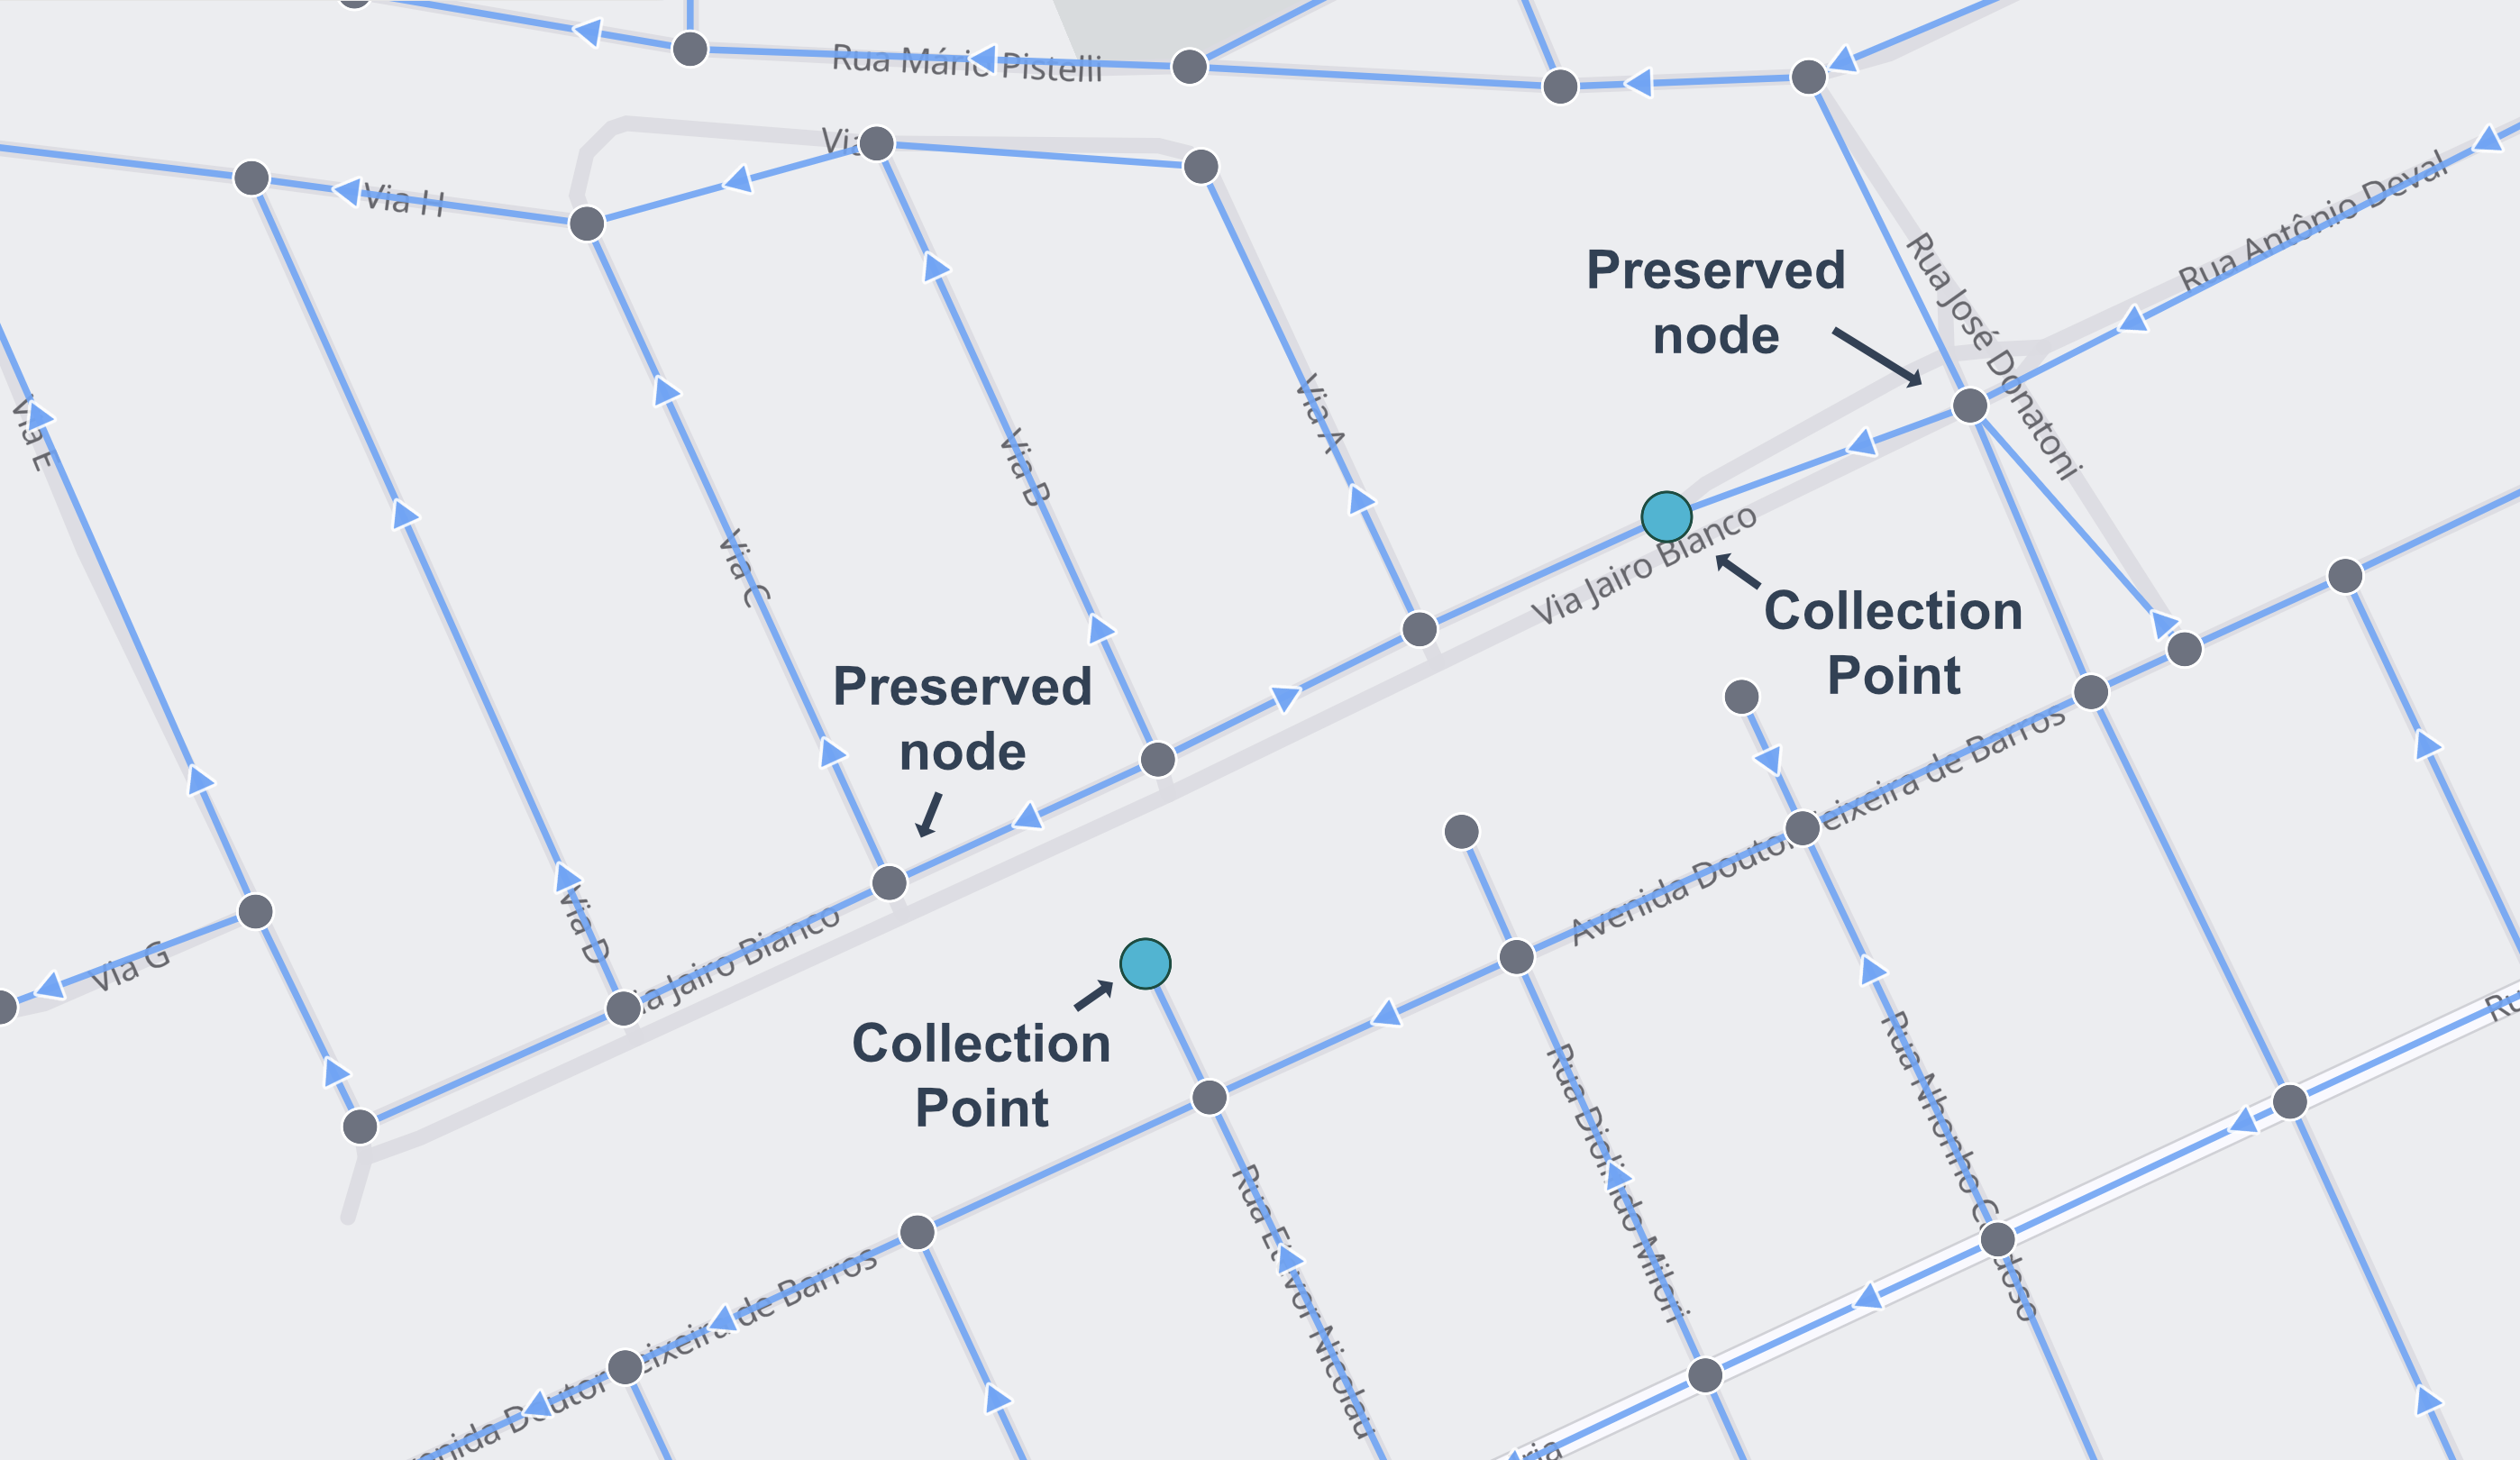
\includegraphics[width=\linewidth]{images/post-processed.png}
    \end{minipage}
\caption{Local graph example before processing on the left and after sewer-network processing on the right.}
\label{fig:before-after-processing}
\end{figure}

The current validation is functional.
It verifies whether internal steps produce coherent structures: street extraction, elevation enrichment, graph construction, editing, persistence, routing, coverage preservation, and visualization of the processed network.
This includes automated tests for geographic calculations, area validation, node rules, parity between implementations, classification, sanitization, extrema detection, edge cost, RSPH, coverage repair, cycle prevention, elevation handling, and node reduction.


\subsection{Building detection with DL models}

Table~\ref{tab:seg_results} compares the segmentation results obtained before and after fine-tuning each model: SAM and DeepLab V3.
Both models were fine-tuned on the Massachusetts Buildings Dataset using 151 images of $1500 \times 1500$ pixels, tiled into $512 \times 512$ patches with a stride of 256 pixels.
The dataset was split into 137 training, 10 validation, and 4 test images.
Fine-tuning produced substantial gains in both models.
Figure \ref{fig:SAM-finetuned-results} shows examples of segmentation outputs.
SAM improved its mean IoU from 0.160 to 0.586, while DeepLab~V3 increased from 0.177 to 0.600, reaching a mean Dice of 0.747.
These values indicate segmentation quality sufficient to feed sewage contribution estimates into the URBANUS pipeline.
We notice that SAM, originally trained as a general-purpose segmentation model, achieved performance comparable to DeepLab~V3 after fine-tuning, suggesting strong adaptability to the satellite imagery domain.

\begin{table}[ht]
\centering
\caption{Building segmentation results before and after fine-tuning}
\label{tab:seg_results}
\begin{tabular}{lccc}
\hline
\textbf{Model} & \textbf{Fine-tuning} & \textbf{Mean IoU} & \textbf{Mean Dice} \\
\hline
SAM        & No  & 0.160 & --    \\
SAM        & Yes & 0.586 & 0.734 \\
DeepLab V3 & No  & 0.177 & 0.293 \\
DeepLab V3 & Yes & 0.600 & 0.747 \\
\hline
\end{tabular}
\end{table}

\begin{figure}[ht]
    \centering
    \includegraphics[trim={0 0 0 2cm},clip,width=1.\textwidth]{images/SAM-DeepLabV3-comparison.png}
    \caption{Qualitative segmentation results of the fine-tuned SAM versus DeepLab V3 models in the Massachusetts Buildings Dataset.}
    \label{fig:SAM-finetuned-results}
\end{figure}

\subsection{Case study: Verdelândia, MG}

To evaluate the practical utility of \method, a case study was conducted on the Barreiro do Rio Verde neighborhood in the municipality of Verdelândia, Minas Gerais, Brazil.
The city was selected due to its low Human Development Index (HDI of 0.58) and its irregular terrain, both representative of the context for which \method is designed.
The case study covered 21 street alignments, drawn from a total of 242 in the municipality.

A domain expert performed the network planning manually using the same input data as \method, ensuring a fair comparison.
The manual process comprised four stages: (i)~data preprocessing, including file cleanup and longitudinal profile generation for each alignment;
(ii)~manual placement of manholes (PVs) at intersections and topographic inflection points, with identification of high and low points to determine flow direction;
(iii)~hydraulic validation, consisting of filling spreadsheets with sewage contribution, flow rates, hydraulic radius, flow velocity, and tractive stress for each pipe segment;
and (iv)~correction and re-validation of segments that did not meet design constraints.

The total time estimated for the expert to complete the 21 alignments was approximately two weeks of working days, broken down as follows:
file import and cleanup (approx. 2.5~h), high/low point identification (approx. 3.5~h), manhole and pipe placement (approx. 1.5~h), parameter transcription to spreadsheet (approx. 6~h), and verification and corrections (approx. 6~h).
Extrapolating to the full 242 alignments of the municipality, the expert estimated approximately six months of work under normal working conditions.

For the same 242 alignments, the total data-entry and processing time in \method was approximately 41 seconds.
This represents a reduction of several orders of magnitude relative to the expert baseline, without the risk of transcription errors inherent to manual spreadsheet-based workflows.
The building detection module was not validated in this use case: the entry of each building lot was provided manually by the specialist.

Beyond processing time, the case study evaluated the geometric accuracy of the node placement produced by \method.
Two algorithmic steps were assessed against the expert solution used as ground truth.
The first step, which enforces a minimum spacing of 100~m between manholes as required by design standards, achieved 100\% precision across all 21 tested alignments.
The second step, which clusters nearby nodes and merges them into a single representative corner node, achieved a precision of 89.5\% on the same alignments.
These results indicate that \method produces geometrically sound preliminary layouts suitable for further specialist refinement.


